\chapter{Experimental Results}

The Landsat 8 dataset contains 5154 images. The model was trained with 4124 random images and it was tested with 515 random images in the dataset. The performance measuring criterias are 'accuracy', 'precision', 'recall', 'IOU' and 'loss function' for the model's evaluation. 

Several experiments were carried out to determine the best functions and parameters for training and testing the model with Landsat 8 data. 100 images was used for experiments. An owerview of the experiments and their results are provided below:

\begin{itemize}
    \item \textbf{U-Net Architecture Transformation:}\\
    
        The U-Net design was updated by adding an extra convolution function to each of the initial U-Net function's ten convolution layers. In this modification, the first convolution function received the result from the previous layer, while the second convolution function took the convoluted layer as a parameter. The new U-Net architecture was employed for both model training and testing, utilizing a dataset of 100 images. The results demonstrated that the Intersection over Union value decreased from 0.30 to 0.23, while the accuracy increased from 0.54 to 0.76.
        \\
    \item \textbf{Modifying Parameters in the U-Net Architecture:}\\
    
        In the U-Net design, the convolution function contains numerous hyperparameters, one of which is "kernel size." The kernel size is the size of the iterating window over the image during the convolution operation.

        The size of the kernel influences the information acquired by the convolutional layer. Larger kernel sizes can capture more global information, whereas lower kernel sizes can hold more local details.

        Two U-Net designs were trained and evaluated to identify the optimal kernel size for a specific set of data. One architecture used a kernel size of 3, while the other used a kernel size of 5.
        
        Increasing the kernel size from 3 to 5 resulted in a modest improvement in the Intersection over Union value, which improved from 0.30 to 0.31. Yet, there was a minor drop in accuracy, which decreased from 0.54 to 0.53.
        
        These findings indicate that the kernel size chosen might have a minor impact on the performance of the U-Net model, and it is critical to evaluate the trade-off between capturing global information and conserving local features when picking the kernel size for a specific dataset.
        \\
    \item \textbf{Modifying Optimization:}\\
        
        In the U-Net model, the compile function is used to prepare the model for training. There are three parameters required: optimizer, loss, and metrics.

        The optimizer is an optimization technique that determines how the weights of the model are changed during training. One of the optimizer's key parameters is the "learning rate." The learning rate is a hyperparameter that determines the size of the steps used to update the model's weights during training. It has an effect on how quickly or slowly the model learns from training data. A lower learning rate provides greater stability and the possibility of optimal solutions, whereas a higher learning rate allows for faster convergence.
        
        Three U-Net topologies were trained and tested to identify the best learning rate for a given dataset. Each architecture employed a distinct learning rate: 1e-3, 1e-4, and 1e-6.
        
        The results revealed that a learning rate of 1e-6 was insufficient for the model. With this learning rate, the precision and recall scores were approximately zero, indicating poor performance. Learning rates of 1e-3 and 1e-4, on the other hand, were more appropriate for the model. The IOU values obtained were 0.33 and 0.30, with corresponding accuracies of 0.55 and 0.54.
        
        These findings emphasize the significance of choosing an adequate learning rate while training the U-Net model. Both 1e-3 and 1e-4 performed better than the extremely low learning rate of 1e-6, demonstrating the importance of establishing the correct balance between learning speed and accuracy.
        \\
        \\
    \item \textbf{Modifying Compile Parameters:}\\
        \\
        The compile function in the U-Net model is used to prepare the model for training. Three parameters are required: optimizer, loss, and metrics.

        Loss function is the function that calculates the discrepancy between the ground truth and the predicted output of the model. The evolution metric is a parameter used to monitor the model's performance throughout training and testing. The accuracy metric is the most commonly used. It calculates the percentage of correctly predicted classes out of all samples for each sample. The binary accuracy metric computes correct predicted labels from all samples. 

        Four different compile functions were used for training and testing to determine the best compile parameters for a specific dataset. Binary cross entropy and dice loss functions were among the loss functions considered. Similarly, the metrics chosen included accuracy metrics and binary accuracy metrics. The goal of experimenting with different combinations of these four parameters was to find the compile function that produced the best results for the given dataset.

        The results showed that using the dice loss function and binary accuracy metric produced the highest IOU and accuracy values. In particular, the IOU value for the given dataset was 0.76, while the accuracy was 0.84.
\end{itemize}

All examination outcomes demonstrated the optimal U-Net architecture and compile function parameters. The features and parameters were determined after thorough examinations. The learning rate parameter in the optimization function was specifically set to "1e -4," while the kernel size was set at 3. Convolution layers were also implemented to the U - Net function. One of the compile function's parameters, the loss function, was set to the dice loss function. Similarly, the compile function's evaluation metric parameter was set to the binary accuracy metric. As a result, significant improvements in the acquired findings were pointed out.


The accuracy of the training and evolution is 0.91. The result outcomes after evaluation of the model are shown below in Figure \ref{res1}, Figure \ref{res3}.

Black pixels show the absence of clouds, whereas white pixels show the presence of clouds. The resulting image uses purple pixels to represent areas that are inaccurately detected in the prediction. When the pixel is black in the ground truth but white in the prediction then it is purple in the result. The same place is represented by these pixels. In contrast, green pixels show regions that are mistakenly identified as non-overcast in the prediction while being cloudy in the ground truth.
\hfill \break
\begin{figure}[htp]
    \centering
    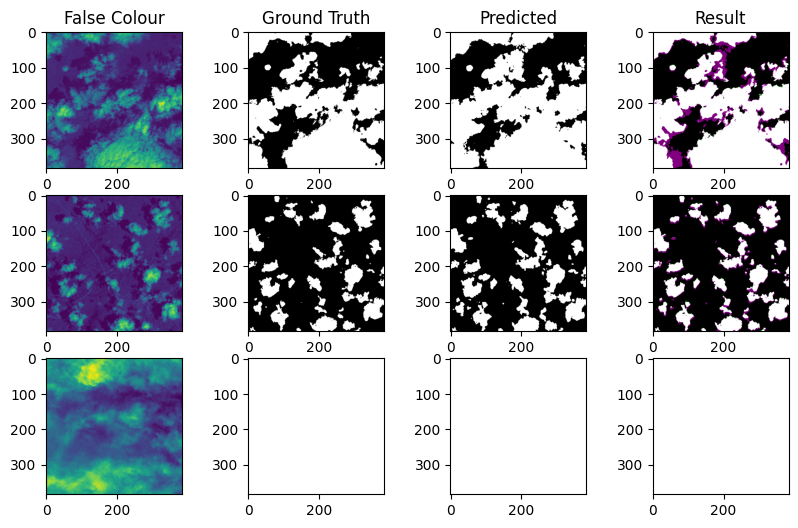
\includegraphics[width=15cm]{projectChapters/images/result1.png}
    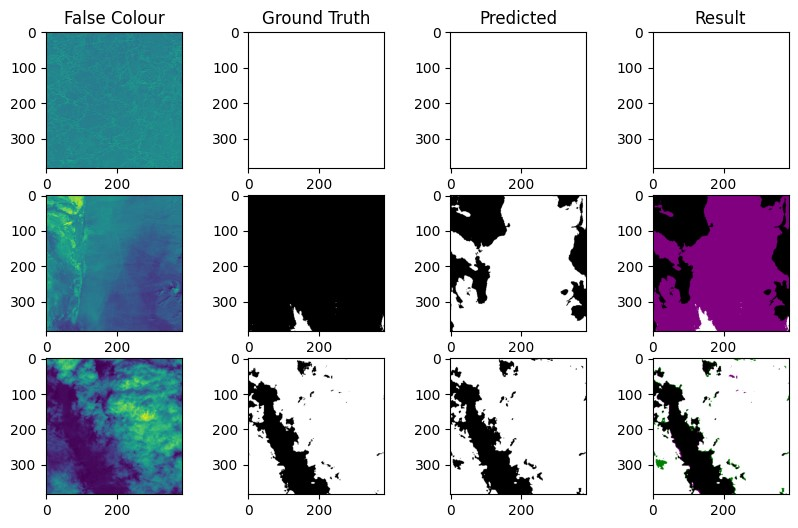
\includegraphics[width=15cm]{projectChapters/images/result2.png}
    \caption{Result Table 1}
    \label{res1}
\end{figure}


\begin{figure}[htp]
    \centering
    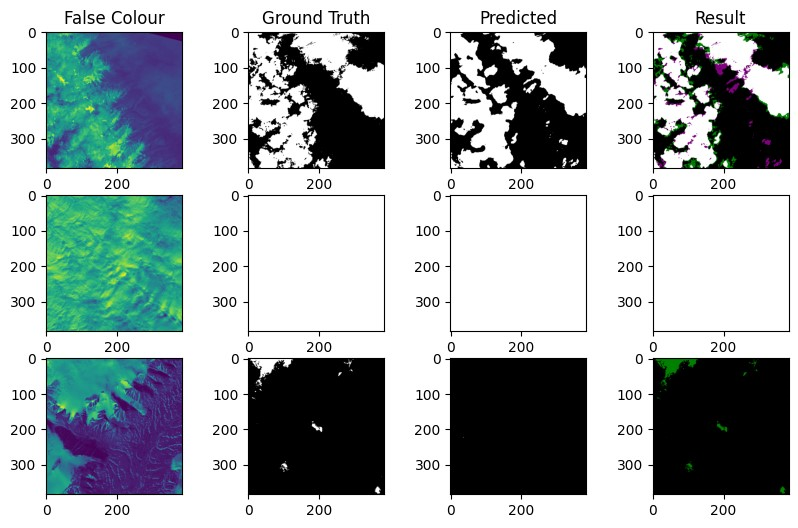
\includegraphics[width=15cm]{projectChapters/images/result3.png}
    \caption{Result Table 2}
    \label{res3}
\end{figure}
\newpage
The success measurements obtained from training and evaluating the model are provided in Table \ref{resultTable}.
\hfill \break
\begin{table}[htp]
    \centering
    \begin{tabular}{ |p{6cm}||p{2cm}|}
     \hline
     \hline
     Performance Criteria & Value\\
     \hline
     \hline
     IOU     &   0.8305\\
     \hline
     Precision   &     0.9309\\
     \hline
     Recall  &  0.9056\\
     \hline
     Binary Accuracy       &     0.9162\\
     \hline
     Loss &   0.2952\\
     \hline
    \end{tabular}

    \caption{Performance Criteria - Value}
    \label{resultTable}
\end{table}
